\section{Trust Evaluation Metrics Based on Technological Parameters}

Anomalous misbehavior of a smartphone may be due to malicious exploit 
of an application, the operating system, or the hardware. In order to 
detect these anomalies, we first need to establish baseline 
measurements for normal behavior. In this paper, we complement the 
standard debugging and anomaly detection techniques and focus on 
metrics that could be obtained without inspection of the app’s source 
or binary code because obfuscation techniques are very sophisticated 
and will continue to be developed.
We have enhanced some existing debugging techniques with additional parameter measurements to inspect app behavior.
The three that we chose are battery voltage, CPU usage, and network usage, which are easy to collect.
The following subsections describe how these three measurements can be linked to specific applications
and can be used to monitor their behavior and, therefore, adjust their trust evaluations.


\subsection{Battery voltage}
The battery voltage is a proxy metric for the amount of remaining 
energy in the battery. Any kind of activity on the device will result 
in a change of battery voltage, but the resolution of readings (both 
in time and in voltage) only allows for coarse, averaged measurements 
under general, non-lab conditions.
If the circumstances can be controlled tightly, then approaches like 
\textit{Eprof} \cite{pathak2012fine} can be used to estimate energy consumption 
of individual activities and assign credit to likely originators.  In the following experiment,
the battery voltage was measured both with and without video ads.
The ​baseline is the battery consumption for a music app.
This was recorded for 15 seconds and 60 seconds.  Then, the measurement was repeated
with both video ads and the music app.  The video ads were only running for the first 15 seconds.
The smartphone consumes only 31.5mA with no apps running, and 56.5 mA with the music app
running.
However, when playing a video ad, the consumption is 169.5mA. 
In the experiment, the video ad lasted 15 seconds.
Over the first 15 seconds, the average battery use attributed to the video ads was 81\% of the total
battery use.  This is very significant and would be difficult to disguise.
The data is shown in Table~\ref{table:battery}.



\begin{table}%[ht]
\centering 
\scriptsize
\caption{A comparison of battery use with anomalous adware compared with normal.
The ad was 15 seconds.}
\label{table:battery}
\begin{tabular}{|l||l|l|}
    \hline
    {\bf Time} & {\bf 15s} & {\bf 60s}  \\
    \hline
    \% of total battery use with ads (avg)  & 81.4\%   & 53.0\%    \\
    \hline
    \% of total battery use with ads (max) & 86.0\%  & 61.5\%   \\
    \hline 
\end{tabular}

\end{table}

\subsection{CPU usage}

\begin{figure*}[ht]
\centering
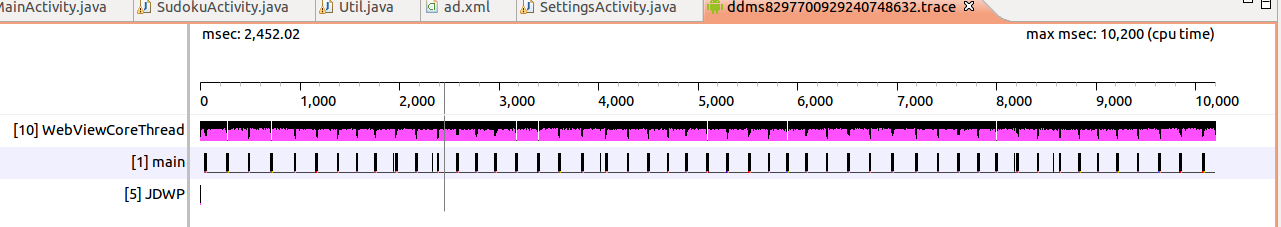
\includegraphics[width=6in]{no_AdsDisplay_10s.png}
\caption{A typical session in Traceview, the execution log viewer.
WebViewCoreThread is busy, but main thread's workload is very light.  main is responsible for 
the user interface, in general.  WebView is responsible for rendering ads using the webkit library}
\label{fig:cpu-no-ad}
\end{figure*}

\begin{figure*}[ht]
\centering
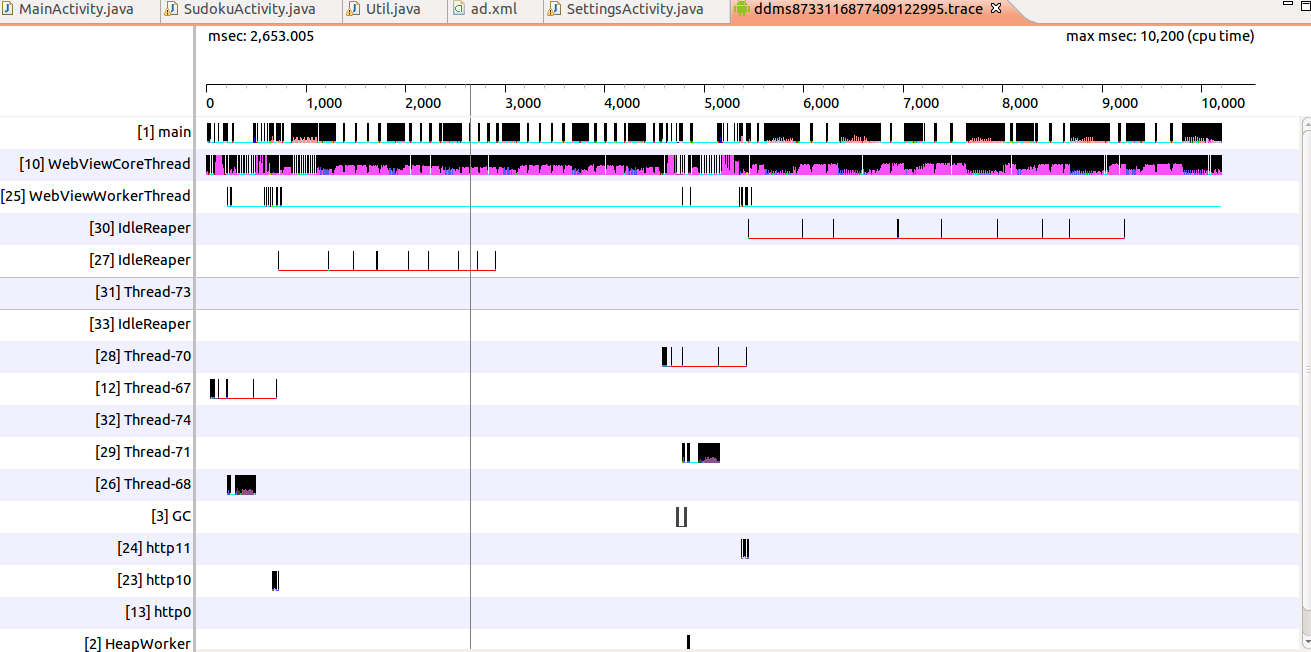
\includegraphics[width=6in]{traceview.png}
\caption{A session in Traceview, with anomalous Ads.  Notice that main is doing much more work and
there are other threads that are getting significant CPU time.}
\label{fig:cpu-ad}
\end{figure*}

Similar to battery voltage, monitoring the overall CPU usage 
(which is an operation requiring no special privileges on Android) 
can be used to get a coarse-grained overview of resource utilization. 
However, the existing debugging and tracing interfaces permit 
finer-grained views as well. Assuming an app is not designed to 
evade or complicate debugging deliberately, the 
\textit{Dalvik Debug Monitoring Service} (DDMS) 
% https://developer.android.com/tools/debugging/ddms.html
provides insight at the system call level\footnote{In computing, a system call is how a program requests a service from an operating system's kernel. This may include hardware-related services (for example, accessing a hard disk drive), creation and execution of new processes, and communication with integral kernel services such as process scheduling~\cite{syscall}.}.  
\eat{Even if an app is trying to evade reverse engineering,
 wouldn't it be hard to eliminate the frequency of syscalls?} % end commment

Figure~\ref{fig:cpu-no-ad} shows a typical  
session in Traceview, an execution log viewer.  The main thread is doing almost all of the work
and making system calls to request resources from the operating system.  Figure~\ref{fig:cpu-ad} shows what happens when a video ad starts 
executing.  There is a dramatic change in activity and the main app thread is no longer 
the primary, uniform consumer of CPU cycles.
% Current figure (MD5 46fbce842e071dfb8f321c9645c6b411) courtesy of Tao Li.
The app under scrutiny comprises several threads with different 
temporal activity patterns. Some threads bear names indicative 
of their performed functions. Colored bars in the threads' activity 
timelines further detail system-call-level interactions with app and system 
libraries, with the height of sub-bars proportional to the frequency 
of specific calls.  
Other log views (not shown) list all of an app's threads, show the 
call stack for each, and display cumulated and individual CPU time 
consumption, and relative usage.


%%% http://www.sigmobile.org/mobisys/2012/program.php#ses5

\subsection{Network usage}

Android provides a number of built-in features that allow the observation 
of a device's network conditions for any app granted the 
\texttt{ACCESS\_NETWORK\_STATE} permission. This permission 
allows applications to access information about networks.
The \texttt{ConnectivityManager} class, an Android class that 
answers queries about the state of network connectivity and 
network connectivity changes, lets an app discover the 
current connectivity status and type (WiFi, 3G, Bluetooth, Ethernet)~\cite{che2011case}. 
For cellular access such as LTE or 3G, the Android \texttt{TelephonyManager} 
class provides access to information about the telephony services on the 
device and thus makes further details available. The stateful nature of cellular 
data connectivity is reflected by various indicators of data activity, 
thereby allowing any app to detect when other apps transfer data over 
the cellular interface.  The Application Resource Optimizer project
(ARO\footnote{See \url{https://github.com/attdevsupport/ARO}}) and \cite{Ricciato2010551} 
provide further insights into what is 
essentially radio resource control (RRC-based type of diagnostics).

%%% https://developer.android.com/reference/android/telephony/TelephonyManager.html (See NETWORK_TYPE_* and DATA_* states)
%%% https://developer.android.com/reference/android/net/ConnectivityManager.html (See TYPE_*)
%%% https://developer.android.com/reference/android/net/NetworkInfo.html#isConnected%28%29

If the device is \textit{rooted} (i.e., system-level administrator 
privileges are granted to the user launching an app), standard 
packet tracing tools such as \texttt{tcpdump} can be used to 
record the exact data transferred across network interfaces. 
However, the precondition is not met on almost any commercial stock 
firmware.
% Note: tcpdump doesn't allow inspection of encrypted content either. 
% There are approaches adding a system-level certificate to MITM on 
% HTTPS connections see for instance https://github.com/egirault/googleplay-api ,
% but I think this also requires root.

When packet-level tracing on the device is infeasible, the network 
connection of the device might be tapped instead. A natural place 
for this would be a WiFi router acting as the device's gateway. 
Neither on-device nor on-path packet tracing allow decryption of 
HTTPS and other encrypted network traffic. However, at least for 
HTTPS implementations using the system libraries, deliberate 
man-in-the-middle (MITM) attacks on traffic may be performed 
by adding a self-provided certificate to the system's certificate 
storage, and redirecting outgoing HTTPS traffic to a local proxy 
server using that certificate.
